\scanpage{20}
% L1–3
\diagram{\begin{tikzcd}[ampersand replacement=\&,row sep=small,column sep=small,execute at end picture={\draw[thin,rounded corners=12pt] ([xshift=-3pt]upperu.north west) -- ([xshift=-4pt]baseone.south west) -- (basetwo.south east) -- ([xshift=4pt]doubleu.east) -- ([xshift=5pt]sheaves.north east);}]
U \& |[alias=upperu]| U' \& |[alias=sheaves]| F'_{U'}\to\unsure{G_{U'}|G'_U|G'_{U'}} \& {}\\
X\arrow[r,dash]\arrow[d,dash] \& X'\arrow[d,dash] \ {\scriptstyle F'} \& X''\arrow[d,dash] \& |[alias=doubleu]| U'' \& F''_{U''}\to G''_{U''}\\
Y \& |[alias=baseone]| Y'\arrow[l,"\mathrm{fpqc}"'] \& |[alias=basetwo]| Y''\arrow[l,shift left=1.4]\arrow[l,shift right=1.4] \& Y'''\arrow[l,dash]\arrow[l,dash,shift left=2]\arrow[l,dash,shift right=2]
\end{tikzcd}}
% L4–7 left
\diagram{\begin{tikzcd}[ampersand replacement=\&,row sep=small,column sep=small]
U \& U' \& G'_{U'}\leftarrow F'\\
\& X'\arrow[dl,"\mathrm{fpqc}"']\arrow[ddl,bend left=60]\quad F' \&\\
X\arrow[d] \& F \&\\
Y \& \&
\end{tikzcd}}
% L4–6 right
pour tt $n$
\[
\begin{aligned}
&\exists J\unsure{\in|=}\{i_1\unsure{-|,\ldots,}i_{\unsure{r|n}}\}\subset I\\
&\unsure{\mathfrak R|\mathfrak r|\mathfrak A}_n\subset\operatorname{Ker}
\left(\underbrace{\widehat O_{Y,y}}_{A}\to\prod_{\alpha\in J}\underline O_{Y_{i_\alpha},y_{i_\alpha}}\right)
\subset\tikz[baseline=(power.base)]\node[draw,rounded corners=8pt,inner sep=2pt](power){$\widehat m_y^{\,n}$};
\end{aligned}
\]
% L6 right
OPS les $Y_i$ artiniens
% L7 right
\diagram{\begin{tikzcd}[ampersand replacement=\&,column sep=small,row sep=small]
{} \& A\arrow[r] \& \underline{A/\mathfrak R_n}\arrow[r,hook] \& \prod\underline O_{Y_\alpha,y_\alpha}\\
Z'_{\deleted{\unsure{\alpha}}}\quad Z'_i \&
\left\{\begin{gathered}Z'_i\cap U'_y\ne\varnothing\\
\text{i.e. }Z'_i\cap X'_y\ne\{x'\}\end{gathered}\right.\arrow[urr,bend right=23] \& \& {}
\end{tikzcd}}
% L9–11
\diagram{\begin{tikzcd}[ampersand replacement=\&,row sep=small,column sep=small]
G_{U'} \& U'\subset \& X'=X^{h}\arrow[d] \& X'_y\arrow[d]\supset U'_y\\
G_U \& U\subset \& X \& X_y\supset U_y\\
\& Z_{\unsure{\alpha_1|a_1|\alpha}} \& \&
\end{tikzcd}}
% L12–13 lower sketches
\figure{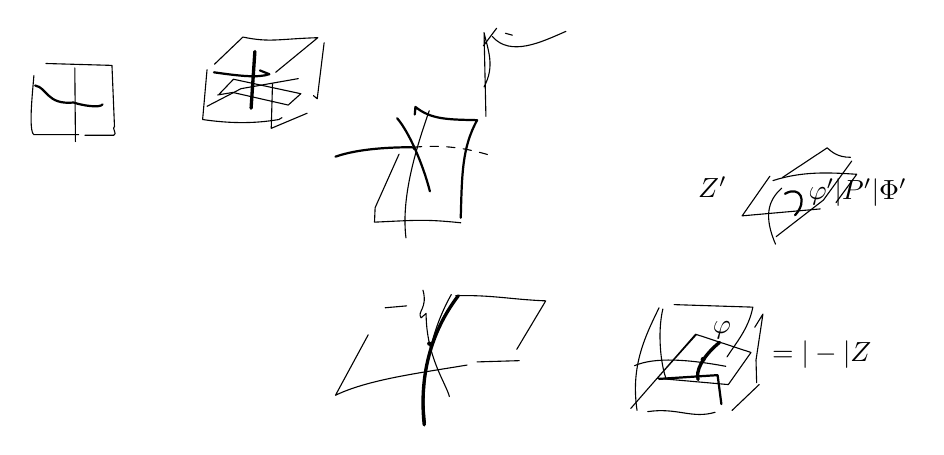
\begin{tikzpicture}[x=.008cm,y=-.008cm,line cap=round,line join=round]
\draw (244,1269) -- (349,1272) -- (353,1369) .. controls (348,1371) and (358,1381) .. (352,1383) -- (306,1383);
\draw (296,1382) -- (225,1382) .. controls (216,1376) and (223,1314) .. (225,1288);
\draw (290,1276) -- (291,1393);
\draw[thick] (227,1304) .. controls (246,1307) and (245,1335) .. (288,1331) .. controls (303,1336) and (330,1340) .. (334,1334);
\draw (512,1270) -- (557,1227) .. controls (600,1236) and (613,1230) .. (676,1228) -- (609,1283);
\draw (686,1236) -- (675,1325) -- (669,1320);
\draw (500,1279) -- (493,1358) .. controls (534,1364) and (573,1365) .. (614,1358) -- (619,1355);
\draw (604,1301) -- (602,1372) -- (659,1348);
\draw[thick] (511,1283) .. controls (553,1289) and (581,1292) .. (599,1286) -- (584,1280);
\draw[very thick] (576,1250) -- (570,1340);
\draw (500,1337) -- (554,1309) -- (645,1293);
\draw (519,1318) -- (542,1294) -- (649,1317) -- (629,1335) -- (541,1315) -- (517,1319);
\draw[thick] (704,1417) .. controls (741,1404) and (793,1402) .. (826,1402);
\draw[dashed] (828,1402) .. controls (885,1397) and (921,1406) .. (957,1417);
\draw (805,1413) -- (767,1498) -- (766,1521) .. controls (832,1518) and (845,1516) .. (903,1522);
\draw[thick] (903,1514) .. controls (905,1444) and (905,1403) .. (929,1359) .. controls (882,1358) and (856,1358) .. (831,1338) -- (830,1350);
\draw (853,1344) .. controls (826,1420) and (809,1489) .. (816,1546);
\draw[thick] (802,1356) .. controls (821,1378) and (843,1429) .. (854,1472);
\fill (829,1404) circle[radius=.024cm];
\draw (943,1353) -- (940,1220) .. controls (946,1247) and (958,1273) .. (940,1306);
\draw (939,1241) -- (960,1213);
\draw (953,1226) .. controls (982,1259) and (1031,1235) .. (1070,1218);
\draw (974,1221) -- (985,1224);
\node at (1303,1465) {$Z'$};
\draw (1394,1448) -- (1350,1511) -- (1474,1500);
\draw (1399,1455) .. controls (1445,1440) and (1488,1442) .. (1532,1445) -- (1499,1490);
\draw (1414,1450) -- (1485,1403) .. controls (1492,1409) and (1501,1418) .. (1522,1418);
\draw (1524,1424) -- (1479,1486) -- (1404,1544);
\draw (1413,1467) .. controls (1391,1486) and (1384,1512) .. (1403,1556);
\draw[thick] (1418,1476) .. controls (1442,1462) and (1455,1487) .. (1434,1510);
\node[right] at (1440,1474) {$\unsure{\varphi'|P'|\Phi'}$};
\draw (783,1657) -- (817,1654);
\draw (756,1700) -- (704,1796) .. controls (756,1771) and (835,1761) .. (913,1748);
\draw (929,1743) -- (996,1741);
\draw (992,1723) -- (1038,1646) .. controls (984,1644) and (950,1636) .. (895,1638);
\draw[very thick] (899,1638) .. controls (854,1697) and (837,1768) .. (845,1843);
\draw (888,1636) .. controls (849,1705) and (840,1786) .. (847,1840);
\draw (843,1629) .. controls (851,1658) and (833,1663) .. (840,1673) -- (848,1666) .. controls (848,1734) and (879,1776) .. (885,1798);
\fill (853,1714) circle[radius=.027cm];
\draw (1218,1657) .. controls (1194,1706) and (1173,1751) .. (1183,1820);
\draw (1224,1659) .. controls (1215,1697) and (1221,1748) .. (1229,1769);
\draw (1242,1652) -- (1367,1656) .. controls (1360,1691) and (1340,1713) .. (1326,1735);
\draw (1179,1749) .. controls (1211,1735) and (1265,1739) .. (1324,1750);
\draw (1173,1817) -- (1276,1699) -- (1364,1728) -- (1328,1779) -- (1215,1769) -- (1277,1700);
\draw (1370,1688) -- (1383,1667) -- (1372,1740) -- (1373,1776);
\draw (1377,1779) -- (1334,1820);
\draw (1200,1822) .. controls (1247,1815) and (1270,1834) .. (1307,1823);
\draw[thick] (1218,1770) -- (1311,1764) -- (1317,1810);
\draw[very thick] (1280,1771) .. controls (1276,1758) and (1286,1735) .. (1314,1712);
\fill (1288,1739) circle[radius=.032cm];
\node at (1318,1692) {$\varphi$};
\node[right] at (1382,1731) {$\unsure{=|-|{}}Z$};
\end{tikzpicture}}
% archive sheet number: 19

